\documentclass[convert={density=300,size=1080x800,outext=.png}]{standalone}
\usepackage{tkz-graph}
\usetikzlibrary{arrows,positioning,shapes,shapes.multipart,patterns,mindmap,shadows}
\usepackage{xcolor}
\usepackage{helvet}
\renewcommand{\familydefault}{\sfdefault}

\begin{document}

\begin{tiny}
    \resizebox{10cm}{!}{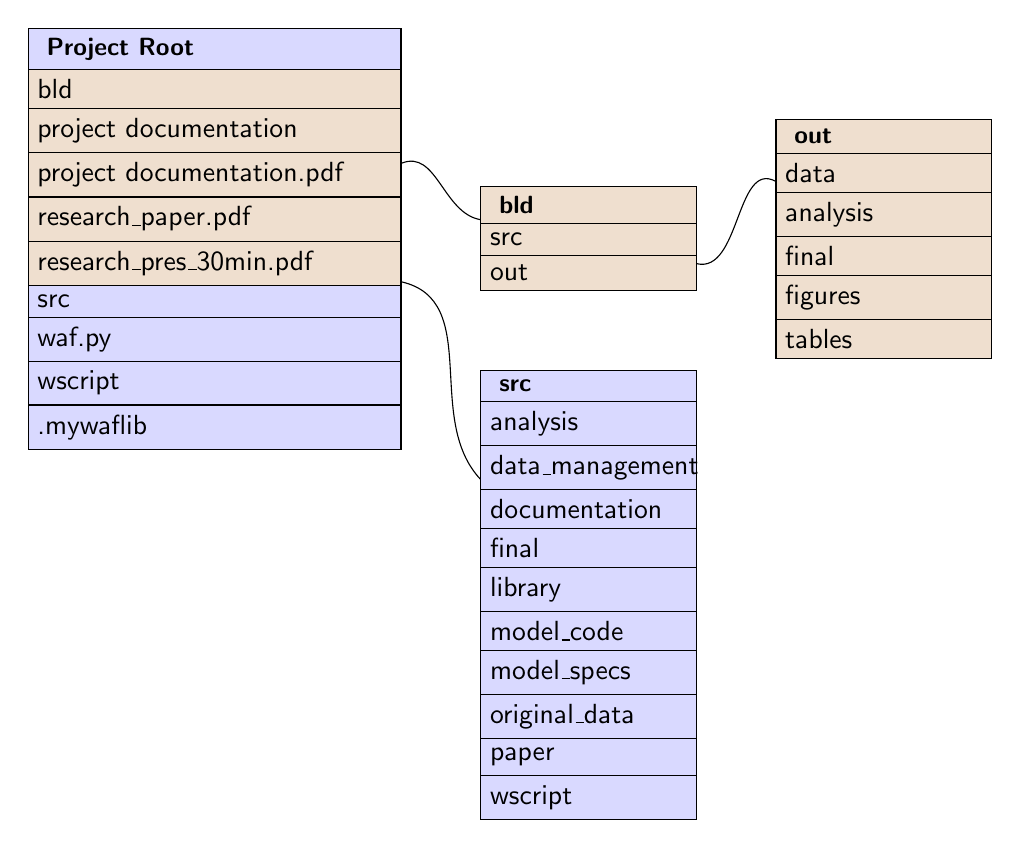
\begin{tikzpicture}[node distance=1cm, auto]
        \node (1) [
            rectangle split,
            rectangle split parts=10,
            rectangle split part fill={
                blue!15,
                brown!25,
                brown!25,
                brown!25,
                brown!25,
                brown!25,
                blue!15,
                blue!15,
                blue!15,
                blue!15
            },
            draw,
            text width=4.50cm
        ]
        {
            \nodepart{one}
                \begin{small}
                    \textbf{Project Root}
                \end{small}
            \nodepart{two}
                bld
            \nodepart{three}
                project documentation
            \nodepart{four}
                project documentation.pdf
            \nodepart{five}
                research\_paper.pdf
            \nodepart{six}
                research\_pres\_30min.pdf
            \nodepart{seven}
                src
            \nodepart{eight}
                waf.py
            \nodepart{nine}
                wscript
            \nodepart{ten}
                .mywaflib
        };

        \node (2) [
            rectangle split,
            rectangle split parts=3,
            rectangle split part fill={
                brown!25,
                brown!25,
                brown!25
            },
            draw,
            text width=2.50cm,
            right=of 1
        ]
        {
            \nodepart{one}
                \begin{small}
                    \textbf{bld}
                \end{small}
            \nodepart{two}
                src
            \nodepart{three}
                out
        };

        \node (3) [
            rectangle split,
            rectangle split parts=11,
            rectangle split part fill={
                blue!15,
                blue!15,
                blue!15,
                blue!15,
                blue!15,
                blue!15,
                blue!15,
                blue!15,
                blue!15,
                blue!15,
                blue!15
            },
            draw,
            text width=2.50cm,
            below=of 2
        ]
        {
            \nodepart{one}
                \begin{small}
                    \textbf{src}
                \end{small}
            \nodepart{two}
                analysis
            \nodepart{three}
                data\_management
            \nodepart{four}
                documentation
            \nodepart{five}
                final
            \nodepart{six}
                library
            \nodepart{seven}
                model\_code
            \nodepart{eight}
                model\_specs
            \nodepart{nine}
                original\_data
            \nodepart{ten}
                paper
            \nodepart{eleven}
                wscript
        };

        \node (4) [
            rectangle split,
            rectangle split parts=6,
            rectangle split part fill={
                brown!25,
                brown!25,
                brown!25,
                brown!25,
                brown!25,
                brown!25
            },
            draw,
            text width=2.50cm,
            right=of 2
        ]
        {
            \nodepart{one}
                \begin{small}
                    \textbf{out}
                \end{small}
            \nodepart{two}
                data
            \nodepart{three}
                analysis
            \nodepart{four}
                final
            \nodepart{five}
                figures
            \nodepart{six}
                tables
        };

        \draw[-, out=22, in=170] (1) to (2);
        \draw[-, out=-13, in=152] (2) to (4);
        \draw[-, out=-13, in=133] (1) to (3);
    \end{tikzpicture}}
\end{tiny}


\end{document}
